\documentclass[11pt, a4paper,titlepage]{article}
\usepackage[hidelinks]{hyperref}
\usepackage{graphicx}
\usepackage{tabularx}
\graphicspath{{img/}}
\author{Edoardo Giacomello \and Mattia Fontana}
\title{SE2 Requirement Analysis and Specification Document} %Definisce il titolo
\newcommand{\productname}{MyTaxiService }
\newcommand{\image}[1]{
	\begin{center}
		\noindent \includegraphics[width=\linewidth]{#1}
	\end{center}
	}
\newcommand{\link}[2]{\underline{\textbf{\hyperref[#1]{#2}}}}
\newcommand{\linkitm}[1]{\underline{\textbf{\ref{#1}}}}
\begin{document}
%Genera il titolo
\maketitle
%Inserisce tabella dei contenuti
\tableofcontents
\newpage
\section{Introduction}
\subsection{Purpose} This document represents the Requirement Analysis and Specification Document (RASD). The main goal of this document is to completely describe the system in terms of functional and non-functional requirements, analyse the real need of the customer to modelling the system, show the constraints and the limit of the software and simulate the typical use cases that will occur after the development. This document is intended to all developer and programmer who have to implement the requirements, to system analyst who want to integrate other system with this one, and could be used as a contractual basis between the customer and the developer.
\subsection{Scope}
The scope of \productname is to manage a taxi service in a more efficient way, along with an emprovement in the interaction between the customers and the service providers. 
\newline In particular, the following goals have be highlighted by the stakeholders:
\subsubsection{Goals}
	\begin{enumerate}
	\item \label{itm:Goal_PassengerInterface} Providing the passenger a \textit{\link{itm:Desc_SimplifiedAccess}{simplified access}} for making real-time \link{itm:Desc_Request}{requests} for the taxi service, according to appropriate \textit{\link{itm:Desc_UsabilityMetric}{usability metrics}}.
	\item \label{itm:Goal_Reservation} Providing the passenger the possibility to \link{itm:Desc_Reservation}{reserve} a taxi for a later moment.
	\item \label{itm:Goal_Confirmation} Providing the passenger a clear confirmation of the taxi ride he’s requesting for.
	\item \label{itm:Goal_WaitingTime} Providing the passenger an estimation of the \link{itm:Desc_WaitingTime}{waiting time} for a taxi ride.
	\item \label{itm:Goal_TaxiInterface} Providing the taxi drivers a \textit{\link{itm:Desc_SimplifiedAccess}{simplified access}} for receiving and handling transportation requests from the passengers.
	\item \label{itm:Goal_FairManagement} Guaranteeing a fair management of the taxi queue, in term of minimizing the passenger \textit{\link{itm:Desc_WaitingTime}{waiting time}}.
	\item \label{itm:Goal_DeveloperInterface} Providing \textit{\link{itm:Actor_SysDevs}{system developers}}  a programmatic interface to further extend the system.
		\end{enumerate}
\subsubsection{Actors and Stakeholders}
\begin{description}
	\item[Customer] \label{itm:Actor_Customer} The person(s) who requested the developing of the system. Also referred as Government in the assignment text.
	\item[Passenger] \label{itm:Actor_Passenger} The person who avails of the taxi service, in particular those who make a request for a Taxi ride.
	\item[Taxi Driver] \label{itm:Actor_TaxiDriver} The employee which is in charge to meet the passenger and take him to the desired location
	\item[User]\label{itm:Actor_User} General term for describing whoever interacts with the system interfaces. It can be a passenger, a taxi driver, a system developer, a system administrator, etc.
	\item[System Developers] \label{itm:Actor_SysDevs} The persons which are qualified and in charge to extend the present system with additional features or services
	\item[System Administrator] \label{itm:Actor_SysAdmin}: The persons in charge to manage the relationship between the transportation service and the system. For example a system administrator could register new taxi drivers’ profiles, manage the passenger profiles or manage data backups.
\end{description}

\subsection{Definitions, Acronyms, Abbreviations}
\subsubsection{Definitions}
	\begin{description}
		\item[Simplified Access] \label{itm:Desc_SimplifiedAccess} Human-to-Machine interaction that satisfy some usability metrics
		\item[Usability Metric] \label{itm:Desc_UsabilityMetric} Precise measurable requirements that an interface has to satisfy in order to provide an efficient and easy experience to the user.
		\item[Waiting time] \label{itm:Desc_WaitingTime} Time in minutes between the submission of a request and the arrival of a taxi.
		\item[Request \textit{(when made by the passenger to the taxi service)}] \label{Itm:Desc_Request} In this document we refer to a \textit{request} when the passenger's intent is to meet the taxi as soon as possible.
		\item[Reservation] \label{Itm:Desc_Reservation} In this document we refer to a \textit{reservation} when the passenger's intent is to meet the taxi at a precise moment in the future
	\end{description}
\subsubsection{Acronyms}
\subsubsection{Abbreviations}
\subsection{Reference Documents}
	\begin{itemize}
		\item Specification Document: Assignments 1 and 2 (RASD and DD).pdf.
		\item Specification Document:Project Description And Rules.pdf
		\item IEEE Std 830-1998 IEEE Recommended Practice for Software Requirements Specifications.
		
	\end{itemize}
\subsection{Document Overview}
The following part of this document will focus on a deeper analysis of the goals highlighted by the stakeholders in addition to some assumptions that must hold in order to keep the system properties valid. The last part of the document will exhibit the software requirements that resulted from the goals examination along with some scenario and use cases that will offer the stakeholders a better comprehension of the final system.   
\pagebreak
\section{Overall description}
This section will cover the overall description of the product. In particular it will put this product into the perspective of other products or systems. 
\subsection{Product Perspective}
The \productname system will partially replace any former traditional system that is based on phone calls with a new interactive system based on mobile and web interfaces. \newline
The decision of completely dismissing the former phone call system in favor to the new one will be left to the customer, since \productname requires the passengers to access a web interface or a mobile application, which is still generally not accessible by some users.
\newline
The project will therefore consists in releasing a web application and a mobile app which are not integrated with any other existing taxi management service.
The system is created to improve the possibility to connect with the taxi service for requesting a taxi, that is based on phone calls.
With this system, the taxi service can provide a fast and innovative system that allow to manage the user request rapidly, without any loss of time.
Both the mobile application and the web interface are connected to the central system and allow the user to know in real time the waiting time, the taxi occupation and their location, and allows to make a taxi request receiving a rapid response.
The application will furthermore provide a programmatic interface for the integration with future systems and extensions.
\newline

	\image{perspective_schema.png}

\pagebreak
\subsubsection{System Interfaces}
	\begin{enumerate}
		\item \productname mobile application will run on tablets and smartphones
		\item \productname web application will run on every terminal which is provided an internet connection and a web browser
	\end{enumerate}
\subsubsection{User Interfaces}
Both the web and mobile applications will have a similar user interface, rearranged to fit the device screen.
\begin{enumerate}
	\item \textbf{Application for passengers} \newline
	\begin{itemize}
		\item It has to provide a \textbf{login page} that allows users to be recognized by the system, along with a registration form that let the user to sign up to the service and a link for resetting the user password.
		In the home page after the login, it is possible to see the map of the zone in which the user is and the taxis that are nearby, along with a menu for accessing the other functionalities. If a taxi is available, the user can request a ride by selecting the button "Call Now". If a taxi is not available, a text message will display the estimated waiting time and the button will let the user to queue. When the user select the request button, a \textbf{confirmation dialog} will ask the user to insert the precise meeting location and, in the case the user is making a reservation, the meeting time.
		After the user has made a taxi request, the system will show directly in the home page the  estimated waiting time for that request. In the case he has made a reservation, the home page is steal usable for making a request, while clicking on \textbf{"your reservation"} a page will display the current reservation status.
		\item \textbf{Passenger menu}
		\begin{description}
			\item[Home] Shows the home page from which is possible to make a new request or check the arrival time and the taxi code of the pending request.
			\item[Your Reservation] Shows the list of pending reservations along with the status or estimated arrival time/taxi code.
			\item[Reserve a Taxi] Display the \textbf{confirmation dialog} in which the passenger can set the meeting time and location
			\item[Your Account] Lead to the account administration page in which the user can show and edit his account
			\item[Logout] Ends the session and leads to the login page
		\end{description}
	\end{itemize}
	\pagebreak
	\item \textbf{Example of the mobile application for passengers: } \newline
	\image{gui_passenger_login.png}
	\image{gui_passenger_home.png}
	\image{gui_passenger_confirmation.png}
	\item \textbf{Application for System Administrators (Web)}
		\begin{itemize}
			\item From the same \textbf{login page} for the users, system administrators can access the administration page by inserting their login data. \newline
			From the administration panel the user can see the list of all the taxis and their current status.
			From the menu they can access the log page from which it is possible to read all the system history, the account administrator page or the backup/restore facility.
		\end{itemize}
		\pagebreak
		\item \textbf{Example of the web application for administrators: } \newline
		\image{gui_admin.png}
	
	\item \textbf{Application for taxi drivers (Mobile)}
		\begin{itemize}
			\item The taxi drivers have a particular login page that allows them to access by taxi code/email and password. \newline The taxi application interface is as simple as can be, for avoiding loss of time and incomprehensions.
			In the homepage the user can see a map of the newarby area. When a request arrives, the user is notified about the time and location of the request. Two buttons allow to accept/decline the request, and when a request is accepted the taxi driver can state he completed the ride or release the ride for another drive.
		\end{itemize}
		\item \textbf{Example of the mobile application for taxi drivers: } \newline
		\image{gui_driver.png}
	
\end{enumerate}

\subsubsection{Hardware Interfaces}
The \productname mobile application will require a smartphone or tablet and will support the most common screen resolutions. \newline
For the correct functionality of \productname mobile and web application (both for passenger and taxi drivers) the device will be required to support the GPS localization and a WiFi or data internet connection. 
\subsubsection{Software Interfaces}
\begin{itemize}
	\item \productname Application Server
		\begin{itemize}
			\item Database Management System (DBMS):
			\begin{itemize}
				\item[Name]: MySQL.
				\item[Version]: 5.6.19
				\item[Source]: http://www.mysql.it/
			\end{itemize}
			\item Application server:
			\begin{itemize}
				\item[Name]:  Jboss application server J2EE open source.
				\item[Source]: http://www.jboss.org/
			\end{itemize}
			\item Operative Systems:
			\begin{itemize}
				\item: Ubuntu/Debian Linux
				\item: Windows Server, Windows 7, Windows 8, Windows 10
			\end{itemize}
		\end{itemize}
		
	\item \productname Application Server
	\begin{itemize}
		\item Mobile Application
		\begin{itemize}
			\item[OS]: Android 4.4.2 or higher, iOS, Windows Mobile.
		\end{itemize}
	\end{itemize}
	\begin{itemize}
		\item Web Application
		\begin{itemize}
			\item[Web Browsers]: Chrome, Firefox, Safari, Opera, Internet Explorer
			\item[Other]: JRE 1.7 or higher
		\end{itemize}
	\end{itemize}	
\end{itemize}

The internal system must make use of these tecnologies for the internal component interfacing

\subsubsection{Communications Interfaces}
	The communication between the server and mobile application will make use of the following ports:
	\newline \newline
	\begin{tabular}{c c c}
		\textbf{Protocol} & \textbf{Application} & \textbf{Port} \\
		\hline
		TCP & HTTP & 80 \\
		\hline
		TCP & HTTPS & 443 \\
		\hline
		TCP & DBMS & 3306 \\
		\hline
	\end{tabular}
	\newline \newline
	The default communication protocol will be HTTPS. \newline
	The data exchange between the server and the mobile applications will occur by the JSON data format, while the web interface will make use of both JSON and AJAX for the communication between the Web Browser and the server.
		
	\image{schema_communication_interface.png}
	
\subsubsection{Memory Constraints}
The suggested memory requirements are: \newline
\begin{itemize}
	\item Application Server
	\begin{itemize}
		\item[Main Memory]: 4GB
		\item[Secondary Memory]: 2GB
	\end{itemize}
	\item Mobile Application
	\begin{itemize}
			\item[Main Memory]: 500Mb
			\item[Secondary Memory]: 100Mb
	\end{itemize}
\end{itemize}
\subsubsection{Operations}
	In this section will be described what operations each kind of user can do by interacting with the system interface: \newline
	\begin{enumerate}
		\item Passengers (Web and Mobile Application)
			\begin{description}
				\item[Registration] The user can create a new account filling in his personal informations
				\item[Login] The user can access the main page by inserting his email and password.
				\item[Map] The user can visualize the map of the zone he is in.
				\item[Request] The user can request a taxi immediately, or adding to the queue according to the taxi availability
				\item[Reservation] The user can make a reservation of a taxi ride for a later moment
				\item[Pending Reservation] The user can visualize data such the estimated taxi arrival time about the reservation he made and cancel a reservation.
				\item[Information] The user can access some information about the system usage and rules
				\item[Profile] The user can access its profile personal data
				\item[Logout] The user can logout from the system
			\end{description}
			
		\item Taxi Drivers (Mobile Application Only)
			\begin{description}
				\item[Login] The user can access the main page by inserting his taxi code and password. This will state the availability of accepting requests.
				\item[Map] The user can see a map of the nearby area. When a request arrives the map will show the meeting point
				\item[Request Incoming] The user can accept or refuse an incoming request
				\item[Active Ride] The user can complete a ride when the passenger is at his desired location, or release the ride to another taxi driver if some unexpected event occurs.
				\item[Logout] The user can logout from the system and state his unavailability of taking requests.
			\end{description}
	
		\item System Administrators (Web Interface Only)  
			\begin{description}
				\item[Login] The user can login and access the administration page
				\item[Taxi Management] The user can acess the list of all active and unactive taxi accounts. He can Add and Remove taxi driver accounts or change their passwords.
				\item [Account Management] The user can access user profiles to provide support to end users and reset their passwords.
				\item[Logs] The user can view and download the logs associated to each accepted/refused request, all ride data such passenger account, departure/arrival date and location, and the taxi driver who made the ride.
				\item[Backup/Restore] The user can make security backups of account data and restore them.
			\end{description}
		
		\item System Operations
		\begin{description}
			\item[Store user information] Creates or updates a passenger profile
			\item[Store taxi information] Creates or updates a taxi profile
			\item[Update Map] Update the map every 30 seconds with each taxi location
			\item[Registration Confirmation] The system sends a confirmation email to the user upon registration
			\item[Request Confirmation] The system sends a confirmation email about the acceptance of a taxi request
			\item[Reservation Confirmation]  The system sends a confirmation email about the acceptance of a taxi reservation
			\item[Reservation Reminder] The system sends a remainder email to the user who reserved a taxi 2 hour before the meeting time
			\item[Time estimation] The system estimate the time needed to move by car from a location A to a location B. It can make use of external map services for this purpose.
		\end{description}
		
		\item System Support Operation
			\begin{description}
				\item[Backup Database] The system make a backup of the database and logs
				\item[Restore Database] The system make a restore of a previous backup of the database
				\item
			\end{description}
			
	\end{enumerate}
\subsection{Product Functions}
This section will list the general functions of the system, with an eventual reference to the goal they contribute to satisfy.
	\begin{enumerate}
		\item \textit{Relative to goal \linkitm{itm:Goal_PassengerInterface}}: The system shall provide the passengers both a web and a mobile application with equivalent functionalities for requesting a ride
		\item \textit{Relative to goal \linkitm{itm:Goal_TaxiInterface}}: The system shall provide a mobile application for taxi drivers, in which they can inform the system about their availability and confirm or refuse the proposed request.
		\item \textit{Relative to goal \linkitm{itm:Goal_FairManagement}}: The system shall associate a queue of taxis to each zone according to the GPS location of the taxis
		\item \textit{Relative to goals \linkitm{itm:Goal_Confirmation} and \linkitm{itm:Goal_WaitingTime}}: The system shall provide a response to the passenger who requested a ride, the notification will contain the code of the taxi that accepted the request and the estimated waiting time.
		\item \textit{Relative to goal \linkitm{itm:Goal_DeveloperInterface}}: The system shall comprehend a programmatic interface that offer the access for the main functionality of the system itself.
		\item \textit{Relative to goal \linkitm{itm:Goal_Reservation}}: The system interface for passengers shall provide the functionality of taxi reservation for rides that will take place after 2 hours. The information required by the system include the origin and destination and the departure date.
		\item {Relative to goal \linkitm{itm:Goal_FairManagement} and security}: The system shall keep track of any active ride, along with the current taxi position and provide an history.
		\item \textit{Relative to goal \linkitm{itm:Goal_TaxiInterface} and Administration}: The system should provide a web interface for system administrators, in which they can manage the taxi drivers and the passenger profiles
		\item \textit{Relative to goal \linkitm{itm:Goal_Confirmation}} The system sends a remainder email or push notification to the user who reserved a taxi 2 hour before the meeting time, just after that it has assigned a taxi to that request.
		\item \textit{Relative to goal \linkitm{itm:Goal_FairManagement}}: The system should manage exceptional situations such the availability of taxis or accidents/vehicle failures.
		\item \textit{\textbf{Not provided functionality}}: The system will not manage the payment for the taxi, which will occour directly to the taxi driver via cash or credit card and it will be managed separately by the transportation company
		
	\end{enumerate}
\subsection{User charateristics}
	There are 4 types of system users: \newline
	\begin{description}
		\item[passenger] Who access the system for requesting a transportation. For this purpose, the user must have an internet connection on his smartphone or computer. In the case he's using a smartphone, the user can have the \productname application installed or using the web interface. For using the web interface the user must have a compatible browser.
		\item[Taxi Driver] Who provide the transportation to the passengers. The user interacts with the system for receiving transportation tasks. The user will be provided a compatible device in advance, and must be in possess of his login credentials, which are generated by the system and managed by system administrators. 
		\item[System Administrator] Who manages the transportation service. The system administrator is in charge to give support to taxi drivers and passengers, in particular to create and supervise taxi drivers' accounts. It's the only figure that have access to the system logs and taxi managements.
		\item[System Developers] Who is in charge to further extends the system. System developers will make use of this document and the Design document for planning the addition of new functionalities.
	\end{description}
\subsection{Constraints}
\subsubsection{Regulatory Policies}
The system shall comply with the following regulatory policies:
\begin{itemize}
	\item CODICE IN MATERIA DI PROTEZIONE DEI DATI PERSONALI "Decreto legislativo 30 giugno 2003, n. 196"
\end{itemize}
\subsubsection{Reliability Requirements}
	\begin{itemize}
		\item In case of system faliure, the system must be recoverable from a previous backup
		
		\item The system infrastructure (data centers, servers, network infrastructures, etc) must be sized accordingly to the expected user base size. 
		
	\end{itemize}
\subsubsection{Criticality of the application}
The main criticalities of this project are:
\begin{itemize}
	\item The compliance of the interface according to the usability metrics explained in section 3.
	\item The fair management of taxis. In particular the system must not waste resources such as not reallocating unemployed taxi when necessary and must allocate requests according to well defined precedence rules.
\end{itemize}
A failure in one or more of this criticalities will lead to the loss of clients.


\subsubsection{Safety and Security Consideration}
\productname should comply to the serurity statements listed above: \newline
\begin{itemize}
	\item Only logged users can request a taxi ride. This is for preventing any malicious behaviour in which unknown users can make taxi request without making use of the transportation service.
	\item At the time of registration, a user must read and accept any privacy policy about the user data management
	\item The system must undertake to not divulge the user data to third parties, in addition the user data will be used only for the supply of the service
	\item For the reason stated before, the passenger must supply at least:
		\begin{itemize}
			\item Name
			\item Surname
			\item e-mail address
			\item Phone number or Tax Code
			\item Password
		\end{itemize}
		\item While the taxi drivers must supply at least:
		\begin{itemize}
			\item Taxi Code
			\item e-mail address
			\item Phone number or Tax Code
			\item Password
		\end{itemize}
	\item The system should therefore warn the user about the regulation policy about false impersonation.
	\item The system will hash the user password before storing it into the database, preventing unauthorized access in the case of data leak.
	\item The system will ask the user the email address or the phone number in order to reset his password. The new password will be sent on the user e-mail address.
	\item In the case of taxi drivers, the password is generated by the system and it's updated periodically. The taxi drivers will receive their new password by email.
	\item Every request must be associated to the user identity and kept in a log for security reasons and kept available for  judicial authorities.
\end{itemize}
\subsection{Assumptions and Dependancies}
\subsubsection{Assumptions}
	\begin{enumerate}
		\item \label{itm: Assumption_Zones} The city is already divided in Taxi Zones of approximately 2x2 km each. 
		\item \label{itm: Assumption_MobileProvisioning} Taxis or Taxi Drivers are assumed to be in possession of a mobile device that  
			\subitem 1) have GPS functionalities 
			\subitem 2) is capable of establishing an internet connection with the facility in which the system is hosted. In the case one of these assumption does not hold, the Taxi driver must contact his referent in order to solve the issue.
		\item \label{itm: Assumption_NumberOfTaxis} The number of taxi in service are at least equal to the number of zones.
		\textbf{Rationale}: In this way, in the case that a zone queue is empty, an incoming request is guaranteed to forwarded by at least one taxi in an estimable time by propagating the request to adjacent zone and forwarding the request to the nearest first taxi that is available.
		\item \label{itm: Assumption_FormerSystems} The service is currently running a traditional system based on phone calls	
		\item \label{itm: Assumption_Payment} The payment will occur directly to the taxi driver by cash or credit card and it will be managed by the transportation company
		\item \label{itm: Assumption_Destination} The taxi drivers should not know in advance what the ride destination will be. The passenger informs directly the taxi driver about the desired arrival location.
		\item \label{itm: Assumption_OneReservation} The taxi Drivers are supposed to accept one request or reservation at a time.
		\item \label{itm: Assumption_LengthTime} The maximum time length of a ride is 1 hour and 45 minutes.
		\item \label{itm: Assumption_SquareZones} All zones have a square o rectangular shape
		\item \label{itm: Assumption_Coverage} There are no area in which the service operates that are not covered by a zone.
		\item \label{itm: Assumption_Overlapping} Zones do not overlap.
	\end{enumerate}
\pagebreak
\section{Specific Requirements}
\subsection{External Interfaces} %This should be a detailed description of all inputs into and outputs from complement the interface descriptions in 5.2 and should not repeat information
	This section will list the main input/outputs of the system. \newline
	\begin{tabularx}{\textwidth}{| c | X |}
		\hline
		\textbf{Name} & 
		Login
		\\
		\hline
		\textbf{Context} & 
		Login
		\\
		\hline
		\textbf{Description} & 
		A user requests to Login
		\\
		\hline
		\textbf{Source} &
		Passenger
		\\
		\hline
		\textbf{Destination} & 
		System
		\\
		\hline
		\textbf{Relations} & 
		None
		\\
		\hline
		\textbf{Channel} & 
		Internal to application (via Web)
		\\
		\hline
		\textbf{Data Format} & 
		\begin{itemize}
			\item email: string
			\item password: string
		\end{itemize}
		\\
		\hline		
	\end{tabularx}	
	\begin{tabularx}{\textwidth}{| c | X |}
		\hline
		\textbf{Name} & 
		TaxiProbe
		\\
		\hline
		\textbf{Context} & 
		Taxi Request or Reservation
		\\
		\hline
		\textbf{Description} & 
		The passenger application retrives informations on taxi availability
		\\
		\hline
		\textbf{Source} &
		Passenger Application
		\\
		\hline
		\textbf{Destination} & 
		System
		\\
		\hline
		\textbf{Relations} & 
		None
		\\
		\hline
		\textbf{Channel} & 
		Internal to application (via Web)
		\\
		\hline
		\textbf{Data Format} & 
		\begin{itemize}
			\item User Location (GPS)
		\end{itemize}
		\\
		\hline		
	\end{tabularx}
		\begin{tabularx}{\textwidth}{| c | X |}
			\hline
			\textbf{Name} & 
			TaxiProbeResponse
			\\
			\hline
			\textbf{Context} & 
			Taxi Request or Reservation
			\\
			\hline
			\textbf{Description} & 
			The system replies to a TaxiProbe with the current taxi availability informations
			\\
			\hline
			\textbf{Source} &
			System
			\\
			\hline
			\textbf{Destination} & 
			Passenger Application
			\\
			\hline
			\textbf{Relations} & 
			Response to TaxiProbe
			\\
			\hline
			\textbf{Channel} & 
			Internal to application (via Web)
			\\
			\hline
			\textbf{Data Format} & 
			\begin{itemize}
				\item taxisAvailable: boolean
				\item taxiLocations(taxiCode, taxiLocation, isAvailable): list of locations
				\item waitingTime: integer, in seconds
			\end{itemize}
			\\
			\hline		
		\end{tabularx}
	
		\begin{tabularx}{\textwidth}{| c | X |}
			\hline
			\textbf{Name} & 
			TaxiRequest
			\\
			\hline
			\textbf{Context} & 
				Taxi Request
			\\
			\hline
			\textbf{Description} & 
			The user makes a real-time taxi request
			\\
			\hline
			\textbf{Source} &
				Passenger
			\\
			\hline
			\textbf{Destination} & 
				System
			\\
			\hline
			\textbf{Relations} & 
				None
			\\
			\hline
			\textbf{Channel} & 
				Internal to application (via Web)
			\\
			\hline
			\textbf{Data Format} & 
			 \begin{itemize}
				 \item User Email: string
				 \item currentTime: long
				 \item Meeting Location: location
			 \end{itemize}
			\\
			\hline		
		\end{tabularx}
		\begin{tabularx}{\textwidth}{| c | X |}
			\hline
			\textbf{Name} & 
			TaxiReservation
			\\
			\hline
			\textbf{Context} & 
			Taxi Reservation
			\\
			\hline
			\textbf{Description} & 
			The user makes a taxi reservation
			\\
			\hline
			\textbf{Source} &
			Passenger
			\\
			\hline
			\textbf{Destination} & 
			System
			\\
			\hline
			\textbf{Relations} & 
			None
			\\
			\hline
			\textbf{Channel} & 
			Internal to application (via Web)
			\\
			\hline
			\textbf{Data Format} & 
			\begin{itemize}
				\item User Email
				\item currentTime: Timestamp
				\item meetingTime: Timestamp
				\item meetingLocation: Location
				\item arrivalLocation: Location
			\end{itemize}
			\\
			\hline		
		\end{tabularx}
				\begin{tabularx}{\textwidth}{| c | X |}
					\hline
					\textbf{Name} & 
					Confirmation
					\\
					\hline
					\textbf{Context} & 
					Taxi Request or Reservation
					\\
					\hline
					\textbf{Description} & 
					The system confirms a Taxi request or reservation
					\\
					\hline
					\textbf{Source} &
					System
					\\
					\hline
					\textbf{Destination} & 
					Passenger
					\\
					\hline
					\textbf{Relations} & 
					Response to a TaxiRequest or TaxiReservation
					\\
					\hline
					\textbf{Channel} & 
					Email or Internal to application (optional, for push notifications)
					\\
					\hline
					\textbf{Data Format} & 
					\begin{itemize}
						\item User Email
						\item requestId
						\item requestTime: Timestamp
						\item meetingTime: Timestamp
						\item meetingLocation: Location
						\item arrivalLocation: Location
						\item accepted: boolean
					\end{itemize}
					\\
					\hline		
				\end{tabularx}
				
				\begin{tabularx}{\textwidth}{| c | X |}
					\hline
					\textbf{Name} & 
					Notification
					\\
					\hline
					\textbf{Context} & 
					Taxi Request or Reservation
					\\
					\hline
					\textbf{Description} & 
					The system updates the information about a request or a reservation
					\\
					\hline
					\textbf{Source} &
					System
					\\
					\hline
					\textbf{Destination} & 
					Passenger
					\\
					\hline
					\textbf{Relations} & 
					Triggered by a pending reservation or request
					\\
					\hline
					\textbf{Channel} & 
					Email or Internal to application (optional, for push notifications)
					\\
					\hline
					\textbf{Data Format} & 
					\begin{itemize}
						\item User Email
						\item requestId
						\item requestTime: Timestamp
						\item meetingTime: Timestamp
						\item meetingLocation: Location
						\item arrivalLocation: Location
						\item accepted: boolean
						\item taxiArriving: boolean
						\item taxiCode
						\item waitingTime: integer
					\end{itemize}
					\\
					\hline		
				\end{tabularx}
				
				\begin{tabularx}{\textwidth}{| c | X |}
					\hline
					\textbf{Name} & 
					DriverRequest
					\\
					\hline
					\textbf{Context} & 
					Taxi Request or Reservation
					\\
					\hline
					\textbf{Description} & 
					The system inform the taxi driver of an incoming ride request
					\\
					\hline
					\textbf{Source} &
					System
					\\
					\hline
					\textbf{Destination} & 
					Taxi Driver
					\\
					\hline
					\textbf{Relations} & 
					Triggered by a pending reservation or request
					\\
					\hline
					\textbf{Channel} & 
					Internal to application
					\\
					\hline
					\textbf{Data Format} & 
					\begin{itemize}
						\item requestId
						\item requestTime: Timestamp
						\item isReservation: boolean
						\item meetingLocation: Location
						\item arrivalLocation: Location (optional)
						\item meetingTime: Timestamp (only if isReservation)
					\end{itemize}
					\\
					\hline		
				\end{tabularx}
				
				\begin{tabularx}{\textwidth}{| c | X |}
					\hline
					\textbf{Name} & 
					DriverResponse
					\\
					\hline
					\textbf{Context} & 
					Taxi Request or Reservation
					\\
					\hline
					\textbf{Description} & 
					The taxi driver accepts or refuses a DriverRequest
					\\
					\hline
					\textbf{Source} &
					Taxi Driver
					\\
					\hline
					\textbf{Destination} & 
					System
					\\
					\hline
					\textbf{Relations} & 
					Response to a DriverRequest
					\\
					\hline
					\textbf{Channel} & 
					Internal to application
					\\
					\hline
					\textbf{Data Format} & 
					\begin{itemize}
						\item requestId
						\item email
						\item requestTime: Timestamp
						\item isReservation: boolean
						\item meetingLocation: Location
						\item arrivalLocation: Location (optional)
						\item meetingTime: Timestamp (only if isReservation)
					\end{itemize}
					\\
					\hline		
				\end{tabularx}
				\begin{tabularx}{\textwidth}{| c | X |}
					\hline
					\textbf{Name} & 
					DriverNotification
					\\
					\hline
					\textbf{Context} & 
					Taxi Request or Reservation
					\\
					\hline
					\textbf{Description} & 
					The taxi driver inform the system he has completed a ride or he is releasing it.
					\\
					\hline
					\textbf{Source} &
					Taxi Driver
					\\
					\hline
					\textbf{Destination} & 
					System
					\\
					\hline
					\textbf{Relations} & 
					Only accepted if an affermative DriverResponse arrived to the system
					\\
					\hline
					\textbf{Channel} & 
					Internal to application
					\\
					\hline
					\textbf{Data Format} & 
					\begin{itemize}
						\item requestId
						\item email
						\item requestTime: Timestamp
						\item currentLocation: Location
						\item isCompleted: boolean
						\item isReleased: boolean
					\end{itemize}
					\\
					\hline		
				\end{tabularx}
				\begin{tabularx}{\textwidth}{| c | X |}
					\hline
					\textbf{Name} & 
					LocationUpdate
					\\
					\hline
					\textbf{Context} & 
					Taxi KeepAlive
					\\
					\hline
					\textbf{Description} & 
					The taxi application inform the system about its location.
					\\
					\hline
					\textbf{Source} &
					Taxi Driver Application
					\\
					\hline
					\textbf{Destination} & 
					System
					\\
					\hline
					\textbf{Relations} & 
					Only possible if the driver is Logged
					\\
					\hline
					\textbf{Channel} & 
					Internal to application
					\\
					\hline
					\textbf{Data Format} & 
					\begin{itemize}
						\item email
						\item currentLocation
					\end{itemize}
					\\
					\hline		
				\end{tabularx}
				\begin{tabularx}{\textwidth}{| c | X |}
					\hline
					\textbf{Name} & 
					NewPassword
					\\
					\hline
					\textbf{Context} & 
					Security
					\\
					\hline
					\textbf{Description} & 
					The system provides the user his new password
					\\
					\hline
					\textbf{Source} &
					System
					\\
					\hline
					\textbf{Destination} & 
					User
					\\
					\hline
					\textbf{Relations} & 
					Only if the password has been Resetted
					\\
					\hline
					\textbf{Channel} & 
					Email
					\\
					\hline
					\textbf{Data Format} & 
					\begin{itemize}
						\item email
						\item newPassword
					\end{itemize}
					\\
					\hline		
				\end{tabularx}


\subsection{Functions} %Functional requirements should deÞne the fundamental actions that must take place in the software in accepting and processing the inputs and in processing and generating the outputs.
This section will list specific functional requirements needed in order to accepting and processing inputs and processing and generating the outputs.
	\begin{enumerate}
		\item \textit{Relative to goal \linkitm{itm:Goal_FairManagement}}: The mobile application for Taxi Drivers shall transmit the taxi GPS location to the system every 30 seconds, in order to keep the taxi queues updated.
		\item \textit{Relative to goal \linkitm{itm:Goal_FairManagement}}: When a taxi becomes available, the system shall store the taxi identifier in the queue of the corresponding zone
		\item \textit{Relative to goal \linkitm{itm:Goal_FairManagement}}: When a request arrives from a certain zone and there is at least one available taxi in that zone, the system shall forward it to the first taxi queuing in that zone.
		\item \textit{Relative to goal \linkitm{itm:Goal_FairManagement}}: Upon an incoming request, If the Taxi Drivers confirms  the system shall inform the passenger, if he doesn’t confirm then the system will forward the request to the next driver in queue and move the taxi driver which refused in the last position in the queue.
		\item \textit{Relative to goal \linkitm{itm:Goal_Confirmation}}: The passenger will be informed of any unexpected event by email if he made the request via the web interface and via email and push notification if he’s using the mobile application. 
		\item \textit{Relative to goal \linkitm{itm:Goal_Confirmation}}: In any case, the passenger can check the request details and information by accessing the web or mobile interface
		\item \textit{Relative to goal \linkitm{itm:Goal_FairManagement}}: If the taxi driver who accepted a request is unable to reach the passenger in a reasonable amount of time (i.e. due to an accident or a vehicle failure) then the taxi driver should be able to release its request. The request is forwarded to the first available taxi and the passenger will receive an update about the new taxi code and the new estimated waiting time.
		\item \textit{Relative to goal \linkitm{itm:Goal_Reservation}}: The reservation request is accepted only if it is made at least two hours before the ride. An earlier reservation should be made impossible to select from the GUI and double checked in the backend.
		\item \textit{Relative to goals \linkitm{itm:Goal_FairManagement} and \linkitm{itm:Goal_Reservation}}:For guaranteeing the precedence of reservation over real-time requests, a reservation is forwarded to a taxi 2 hours before the meeting time: in this way the taxi will result not available for eventual real-time requests (which has a maximum time length, as stated in the assumption \linkitm{itm:Assumption_LengthTime}) that occur in the meanwhile and the request will be forwarded to the next taxi. The taxi is supposed to be at the meeting point at least 10 minutes before the meeting time.
		\item \textit{Relative to goal \linkitm{itm:Goal_FairManagement}}: Along with the taxi queue, there will be a Request Queue, with a FIFO policy. In this way, the first passenger who makes a real-time request is the first that is served by the first available taxi. 
		\item \textit{Relative to goal \linkitm{itm:Goal_PassengerInterface}}: The system should provide passengers a "password reset" service.
		\item \textit{Relative to goal \linkitm{itm:Goal_PassengerInterface}}: The system should let the user cancel a previous reservation he made until 2 hours before the meeting time.
		\item \textit{Relative to goal \linkitm{itm:Goal_Confirmation}}: The system will send notification to a user as soon as the request has been accepted by a taxi driver
		\item The GPS localization of the passenger is used merely for providing a better GUI experience (i.e. showing the right portion of the map) and it is an optional requirement for the passenger. The actual localization occurs by the information that the user provides by inserting the meeting location while making a request.
		\item If the Taxi Driver doesn't reply to a request within a minute, the request is considered refused.	
	\end{enumerate}

	\subsubsection{Exceptions Management}
		In the following diagram will be described the logical flow of steps to follow in some particular cases: \newline
		\image{schema_exceptions.png}
\subsection{Logical Database Requirements}
	This section contains a ER Schema draft for the database, meant for giving the designers a better understanding of the crucial application data.
	\image{schema_database.png}
\subsection{Design Constraints}
 The client application will be a \textbf{thin client}.
\subsubsection{Standard Compliance}
	The mobile application for passenger must comply with the application store regulation policy, depending on the mobile OS for which will be deployed.
\subsection{Software System Attributes}
\subsubsection{Performance Requirements} %Es: 95% of the transactions shall be processed in less than 1 s.
\begin{itemize}
	\item The server shall process the 95\% of operations in less than 1 second.
	\item In optimal network conditions the user shall get a response for a confirmation in less than 5 seconds. This not includes email confirmations. 
\end{itemize}
\subsubsection{Availability}
 Here follows a draft of the interal system phisical architecture, which aids to bettere comprehend the availability analysis.
  \image{schema_availability.png}
 \begin{itemize}
 \item Each database and web application server shall have at least a 3-nine availability.
 \item The load balancer, firewall and application server shall have at least a 5-nine availability since they are crucial for the business process and they are more cost-effective.
\end{itemize}
\subsubsection{Security}
 \begin{enumerate}
 	\item The login information and the user data must be kept safe by the system. In particular, the user data can be accessed only by the user itself or a system administrator, which can see and edit the entire user profile except the password.
 	\item A taxi request or reservation can be made only by registered and logged users, in order to avoid unintentional or malicious requests.
 	\item The transport layer will make use of SSL and HTTP (HTTPS) 
 	\item The passenger password can be reset by inserting the user email. The server will then provide a new temporary password and send it by email to the user.
 	\item The taxi driver password is managed directly by the system and can be resetted only by contacting a system administrator. This is for avoiding disturbance in the case a malevolent user learns about the taxi driver email and tries to reset the taxi driver password. 
 	The taxi driver password is reset every six month and sent automatically to the taxi driver email recipient
 	\item All user password must have a costraint in the number of characters, which will be between 8 and 20.
 \end{enumerate}
\subsubsection{Portability}
	The \productname service will be written in Java. All system modules will have to be developed accordingly to the inherent java portability, in particular the testing phase will comprehend the following systems:
	\begin{enumerate}
		\item Android 4.4 and later
		\item iOS
		\item Internet Explorer, Chrome, Safari, Opera, Firefox
	\end{enumerate}
\subsection{Scenarios}
\begin{enumerate}
	\item Alice is at the Garibaldi railway station, as he has just arrived from Rome.
	She needs a lift to his office as soon as possible, so he decides to look for a taxi.
	On her smartphone she installed the \productname app.
	As soon as she get off of the train, Alice checks the application and control the situation of taxis in the zone of the station, then she requests a taxi service by inserting her position.
	After a few seconds the application replies with the code of a taxi which is near the station.
	When Alice will get out of the station, she will find the taxi with the corresponding code that will take her to his office.
	\item Tomorrow Bob will have to go to the airport, as he has a flight at 23:00.
	He must be at the airport at 21:00 and he need to take a taxi.
	Since he’s at home, Bob decides to register to \productname website from his computer in order to reserve a taxi for the airport. After inserting a few informations he is able to reserve a taxi for the 20:00 of the day after.
	The day after, a taxi driver receives a request at 18:00, the request indicates Bob’s home address and the arrival time which is at 19:50.
	When the taxi drivers accepts the request, Bob receives an email asserting that a taxi is on the way for his home and will be waiting there when he will get out at 20:00.
	\item Carl works for an important society of import-export; today afternoon he will take the plane for going to Usa to close an important deal. His friend Daniel will bring him to the airport.
	Unfortunately his friend had an accident so he can’t bring Giovanni to the airport.
	The inconvenient occurs at 14:30 and Giovanni must be at the airport at 15:30.
	Carl uses the web application to request a taxi at 14:45; but he sees on the web page that no taxis are available in that zone right now, but the nearest available will arrive in 25 minutes. He still decides to queue for a taxi anyway and the system accepts his request.
	\item Kevin is a taxi driver and on his smartphone has installed \productname taxi application.
	He has just done a ride for bring Mrs Thompson from the station to her house.
	As soon as he leave Mrs Thompson and receives the payment, he select the “Ride Completed” button. After a few seconds, a new request arrives.
	He accepts the request and he leaves for the new meeting location.
	\item Samuel is a taxi driver and on his smartphone has installed \productname taxi application.
	He has just done a ride for bring Ms Rossi from the station to her house in the other side of the city.
	When he left her, on his smartphone, a request for a ride arrives.
	As his shift is about to end, he refuses the request and logs out, so the system contacts another taxi driver that accepts the request.
	\item Giovanna is a passenger. Since she hasn’t used the service for a long time, she cannot remember her password, so she press the “forgot password” button in the login page and inserts her email address. After a few seconds the system sends her a new password, that she uses to log-in and access the profile page where she can input a new password inserting the generated password and the new one.
	\item As the trains are on strike, the taxi service is literally overwhelmed by requests.
	Luca wants to request a ride from the station in the zone 1 of the city so he opens the web application home page.
	In his zone there are no taxi available, so the system checks if there’s an available taxi in the other zones but no available taxis are found.\newline 
	Luca sees a notification about that and he decides that he can wait a bit, so he commit request and the system puts that in a queue. \newline
	When a taxi will be available, it will receive the request, and if the taxi driver accepts, Luca will receive an email informing him that a taxi is on the way, along with the estimated waiting time.
	
	
	
\end{enumerate}
\pagebreak
\subsection{State Machines}
	\image{diagram_state_machine1.png}
	\image{diagram_state_machine2.png}
	\image{diagram_state_machine3.png}
	\image{diagram_state_machine4.png}
\subsection{Class Diagram}
	 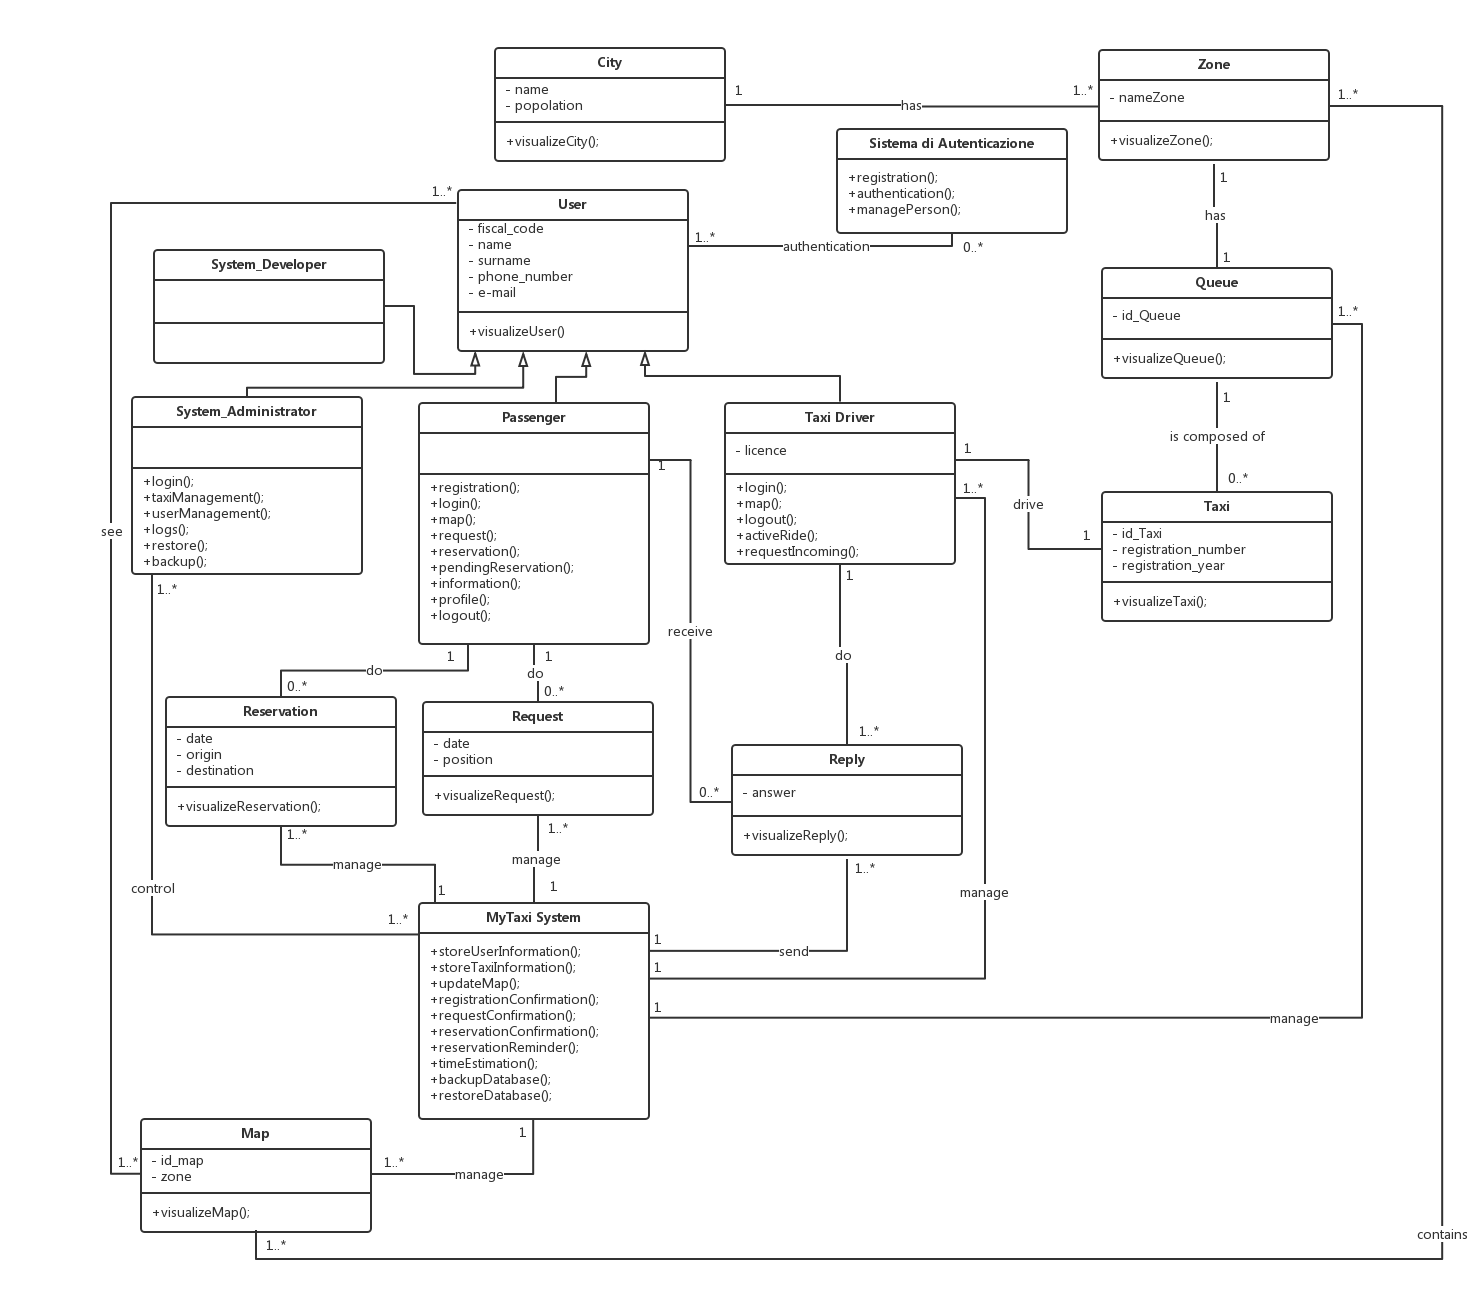
\includegraphics[width=\textwidth]{schema_class_diagram.png}
\pagebreak
\subsection{Use Cases}
\subsubsection{Use Case: General}
	\image{usecase_general.png}
\subsubsection{Use Case: Login}
	\begin{tabularx}{\textwidth}{| c | X |}
		\hline
		\textbf{Name} & 
			Login
			\\
		\hline
		\textbf{Actors} & 
			User (Passenger, Taxi Driver, System Administrator), System 
			\\
		\hline
		\textbf{Entry Conditions} &
			 The user has successfully inserted username and password in the login form 
			\\
		\hline
		\textbf{Flow of events} & 
			\begin{enumerate}
				\item The user goes to the home page of the application.
				\item The user clicks the button “login”.
				\item The user enters his username and password in the form provided
				\item The system shows the private page of the user
				\item The system controls the informations that the user inserts. 
				
			\end{enumerate}						
		\\
		\hline
		\textbf{Exit conditions} & 
			The user clicks on logout. 
			\\
		\hline
		\textbf{Exceptions} & 
			The information inserted in the form is wrong, an error message is shown and so the user re-inserts the information. 
			\\
		\hline		
	\end{tabularx}
	\image{usecase_login.png}
	\image{diagram_sequence_login.png}
	\newpage
\subsubsection{Use Case: Registration}
	\begin{tabularx}{\textwidth}{| c | X |}
		\hline
		\textbf{Name} & 
		Registration
		\\
		\hline
		\textbf{Actors} & 
		User(Passenger), System 
		\\
		\hline
		\textbf{Entry Conditions} &
		The user isn’t registered. 
		\\
		\hline
		\textbf{Flow of events} & 
		\begin{enumerate}
			\item The user clicks on “Registration” button to start the registration process.
			\item The user fills in the form with :
				\begin{itemize}
					\item e-mail
					\item name
					\item surname
					\item cell phone number
					\item tax code
					\item password
					\item verification password
				\end{itemize}
			\item User clicks on “submit” button.
			\item The application will save the data in the DataBase.
			\item User can now enter in the home page and he can make a reservation for a taxi service.	
		\end{enumerate}						
		\\
		\hline
		\textbf{Exit conditions} & 
		The user clicks on cancel or "submit" button. 
		\\
		\hline
		\textbf{Exceptions} & 
		\begin{itemize}
			\item One or more mandatory fields are not valid.
			\item Password not match
			\item Password don't meet the requirements
			\item Email address is already associated to another user.
		\end{itemize} 
		\\
		\hline		
	\end{tabularx}
	\image{usecase_registration.png}
	\image{diagram_sequence_registration.png}

\subsubsection{Use Case: Profile}
	\begin{tabularx}{\textwidth}{| c | X |}
		\hline
		\textbf{Name} & 
		Profile
		\\
		\hline
		\textbf{Actors} & 
		User(Passenger), System 
		\\
		\hline
		\textbf{Entry Conditions} &
		Registered user must be already logged in. 
		\\
		\hline
		\textbf{Flow of events} & 
		\begin{enumerate}
			\item The user clicks on “Profile” button to see the private information that he inserts when he registered to the application.
			\item If user wants to see the information, the system had to store them in the database.
				
		\end{enumerate}						
		\\
		\hline
		\textbf{Exit conditions} & 
		The user clicks on logout or another menu item
		\\
		\hline
		\textbf{Exceptions} & 
		\begin{itemize}
			\item The system can not show the user information.
		\end{itemize} 
		\\
		\hline		
	\end{tabularx}
	\image{usecase_profile.png}
	\image{diagram_sequence_profile.png}
	\newpage
\subsubsection{Use Case: Reservation}
		\begin{tabularx}{\textwidth}{| c | X |}
			\hline
			\textbf{Name} & 
			Reservation
			\\
			\hline
			\textbf{Actors} & 
			User(Passenger), System 
			\\
			\hline
			\textbf{Entry Conditions} &
			Registered user must be already logged to the application. 
			\\
			\hline
			\textbf{Flow of events} & 
			\begin{enumerate}
				\item Passenger clicks on “Reservation” button to request a taxi.
				\item For requesting a taxi the user must insert position and destination of his ride.
				\item The system sends an email to confirm a reservation.
				\item The system sends a reminder e-mail to the user to remind him the taxi  reservation two hours before the meeting time.
			\end{enumerate}						
			\\
			\hline
			\textbf{Exit conditions} & 
			The user clicks on logout or another menu item
			\\
			\hline
			\textbf{Exceptions} & 
			\begin{itemize}
				\item The system can not do a reservation because the request of reservation arrive after the limit time to do a reservation..
			\end{itemize} 
			\\
			\hline		
		\end{tabularx}
		\image{usecase_reservation.png}
		\image{diagram_sequence_reservation.png}
		\newpage
\subsubsection{Use Case: Request}
		\begin{tabularx}{\textwidth}{| c | X |}
			\hline
			\textbf{Name} & 
			Request
			\\
			\hline
			\textbf{Actors} & 
			User(Passenger), System 
			\\
			\hline
			\textbf{Entry Conditions} &
			Registered user must be already logged to the application. 
			\\
			\hline
			\textbf{Flow of events} & 
			\begin{enumerate}
				\item Passenger clicks on “Request” button to request a taxi.
				\item For requesting a taxi the user must insert his position.
				\item The system sends an email to confirm a request when it has a reply of a one taxi driver available for a ride
				
			\end{enumerate}						
			\\
			\hline
			\textbf{Exit conditions} & 
			The user clicks on logout or another menu item
			\\
			\hline
			\textbf{Exceptions} & 
			\begin{itemize}
				\item The system can not answer to the request because no taxi driver are available to reply.
			\end{itemize} 
			\\
			\hline		
		\end{tabularx}
		\image{usecase_request.png}
		\image{diagram_sequence_request.png}
		\newpage
\subsubsection{Use Case: Pending Reservation}
		\begin{tabularx}{\textwidth}{| c | X |}
			\hline
			\textbf{Name} & 
			Pending Reservation
			\\
			\hline
			\textbf{Actors} & 
			User(Passenger), System 
			\\
			\hline
			\textbf{Entry Conditions} &
			Registered user must be already logged to the application. 
			\\
			\hline
			\textbf{Flow of events} & 
			\begin{enumerate}
				\item Passenger clicks on “Pending Reservation” button to see the estimated taxi arrival time about the reservation.
				Passenger can also cancel a reservation.
				The System updates the time estimation for informing the user.
			\end{enumerate}						
			\\
			\hline
			\textbf{Exit conditions} & 
			The user clicks on logout or another menu item
			\\
			\hline
			\textbf{Exceptions} & 
			\begin{itemize}
				\item The user has no pending reservation
			\end{itemize} 
			\\
			\hline		
		\end{tabularx}
		\image{usecase_pending_reservation.png}
		\image{diagram_sequence_pending_reservation.png}
		\newpage
\subsubsection{Use Case: Active Ride}
		\begin{tabularx}{\textwidth}{| c | X |}
			\hline
			\textbf{Name} & 
			Active Ride
			\\
			\hline
			\textbf{Actors} & 
			User(Taxi Driver), System 
			\\
			\hline
			\textbf{Entry Conditions} &
			Registered user must be already logged to the application and he accepted a request
			\\
			\hline
			\textbf{Flow of events} & 
			\begin{enumerate}
				\item Taxi driver clicks on “Accept Request” button to see the information of the ride..
				\item Taxi driver can release the ride to another taxi for problems that block it.
			\end{enumerate}						
			\\
			\hline
			\textbf{Exit conditions} & 
			The user clicks on logout or release the request successfully
			\\
			\hline
			\textbf{Exceptions} & 
			\begin{itemize}
				\item The taxi driver can not release his request, because there aren’t other taxi available in this moment.
			\end{itemize} 
			\\
			\hline		
		\end{tabularx}
		\image{usecase_active_ride.png}
		\image{diagram_sequence_active_ride.png}
		\newpage
\subsubsection{Use Case: Logs}
		\begin{tabularx}{\textwidth}{| c | X |}
			\hline
			\textbf{Name} & 
			Reservation
			\\
			\hline
			\textbf{Actors} & 
			User(System Administrator), System 
			\\
			\hline
			\textbf{Entry Conditions} &
			Registered user must be already logged to the application. 
			\\
			\hline
			\textbf{Flow of events} & 
			\begin{enumerate}
				\item System administrator clicks on “Logs” button to view and download the logs associated to each accepted/refused request, all ride data such passenger account, departure/arrival date and location, and the taxi driver who made the ride.
			\end{enumerate}						
			\\
			\hline
			\textbf{Exit conditions} & 
			The user clicks on logout
			\\
			\hline
			\textbf{Exceptions} & 
			\begin{itemize}
				\item The system can not see all the information because not all of the information are available.
			\end{itemize} 
			\\
			\hline		
		\end{tabularx}
		\image{usecase_logs.png}
		\image{diagram_sequence_logs.png}
		\newpage
\subsubsection{Use Case: User Management}
		\begin{tabularx}{\textwidth}{| c | X |}
			\hline
			\textbf{Name} & 
			Reservation
			\\
			\hline
			\textbf{Actors} & 
			User(System Administrator), System
			\\
			\hline
			\textbf{Entry Conditions} &
			Registered user must be already logged to the application. 
			\\
			\hline
			\textbf{Flow of events} & 
			\begin{enumerate}
				\item The system administrator can access user profiles to provide support to end users and reset their passwords by providing the user email.
				\item The system had to update and store the passenger information.
			\end{enumerate}						
			\\
			\hline
			\textbf{Exit conditions} & 
			The user clicks on logout or another menu item.
			\\
			\hline
			\textbf{Exceptions} & 
			\begin{itemize}
				\item The system can not see all the information because not all of the information are available. 
				\item The user doesn’t exists in the database
				
			\end{itemize} 
			\\
			\hline		
		\end{tabularx}
		\image{usecase_user_management.png}
		\image{diagram_sequence_user_management.png}
		\newpage
\subsubsection{Use Case: Taxi Management}
		\begin{tabularx}{\textwidth}{| c | X |}
			\hline
			\textbf{Name} & 
			Taxi Management
			\\
			\hline
			\textbf{Actors} & 
			User(System Administrator), System  
			\\
			\hline
			\textbf{Entry Conditions} &
			Registered user must be already logged to the application. 
			\\
			\hline
			\textbf{Flow of events} & 
			\begin{enumerate}
				\item The system administrator can access the list of all active and inactive taxi accounts. 
				\item He can also add and remove taxi driver accounts or reset their passwords.
				\item The system had to update and store the taxi driver information.
			\end{enumerate}						
			\\
			\hline
			\textbf{Exit conditions} & 
			The user clicks on logout or another menu item
			\\
			\hline
			\textbf{Exceptions} & 
			\begin{itemize}
				\item The system can not see all the information because not all of the information are available.
			\end{itemize} 
			\\
			\hline		
		\end{tabularx}
		\image{usecase_taxi_management.png}
		\image{diagram_sequence_taxi_management.png}
		\newpage
\subsubsection{Use Case: Request Incoming}
		\begin{tabularx}{\textwidth}{| c | X |}
			\hline
			\textbf{Name} & 
			Request Incoming
			\\
			\hline
			\textbf{Actors} & 
			User(Taxi Driver), System
			\\
			\hline
			\textbf{Entry Conditions} &
			Registered user must be already logged to the application. 
			\\
			\hline
			\textbf{Flow of events} & 
			\begin{enumerate}
				\item The taxi driver can accept or refuse a request that arrive from a passenger. 
				\item The system receives the reply of the taxi driver and inform the passenger if the taxi driver accepted
				
			\end{enumerate}						
			\\
			\hline
			\textbf{Exit conditions} & 
			The user clicks on logout or another menu item
			\\
			\hline
			\textbf{Exceptions} & 
			\begin{itemize}
				\item The system can not send a request to a taxi driver (Driver is offline or connection problem)
				\item No response from the driver				
			\end{itemize} 
			\\
			\hline		
		\end{tabularx}
		\image{usecase_request_incoming.png}
		\image{diagram_sequence_request_incoming.png}
		\newpage
\subsubsection{Use Case: Backup}
		\begin{tabularx}{\textwidth}{| c | X |}
			\hline
			\textbf{Name} & 
			Backup
			\\
			\hline
			\textbf{Actors} & 
			User(System Administrator), System  
			\\
			\hline
			\textbf{Entry Conditions} &
			Registered user must be already logged to the application. 
			\\
			\hline
			\textbf{Flow of events} & 
			\begin{enumerate}
				\item The system administrator makes a security backup of the user information on the database.
				\item The system stores the database in a backup device
			\end{enumerate}						
			\\
			\hline
			\textbf{Exit conditions} & 
			The user clicks on logout.
			\\
			\hline
			\textbf{Exceptions} & 
			\begin{itemize}
				\item No connection with the database
				\item No enough space on device
				\item DBMS failure
			\end{itemize} 
			\\
			\hline		
		\end{tabularx}
		\image{usecase_backup.png}
		\image{diagram_sequence_backup.png}
		\newpage
\subsubsection{Use Case: Restore}
		\begin{tabularx}{\textwidth}{| c | X |}
			\hline
			\textbf{Name} & 
			Restore
			\\
			\hline
			\textbf{Actors} & 
			User(System Administrator), System 
			\\
			\hline
			\textbf{Entry Conditions} &
			Registered user must be already logged to the application. 
			\\
			\hline
			\textbf{Flow of events} & 
			\begin{enumerate}
				\item The system administrator makes a restore of the user information on the database.
			\end{enumerate}						
			\\
			\hline
			\textbf{Exit conditions} & 
			The user clicks on logout or another menu item
			\\
			\hline
			\textbf{Exceptions} & 
			\begin{itemize}
				\item Corrupted Backup
				\item No connection to database
				\item Different data format
			\end{itemize} 
			\\
			\hline		
		\end{tabularx}
		\image{usecase_restore.png}
		\image{diagram_sequence_restore.png}
		\newpage
\subsubsection{Use Case: Information}
		\begin{tabularx}{\textwidth}{| c | X |}
			\hline
			\textbf{Name} & 
			Information
			\\
			\hline
			\textbf{Actors} & 
			User(Passenger), System 
			\\
			\hline
			\textbf{Entry Conditions} &
			Registered user must be already logged to the application. 
			\\
			\hline
			\textbf{Flow of events} & 
			\begin{enumerate}
				\item The passenger can see the information that can help him to request a taxi with  the application.
			\end{enumerate}						
			\\
			\hline
			\textbf{Exit conditions} & 
			The user clicks on logout or another menu item
			\\
			\hline
			\textbf{Exceptions} & 
			\begin{itemize}
				\item Web server failure
			\end{itemize} 
			\\
			\hline		
		\end{tabularx}
		\image{usecase_information.png}
		\image{diagram_sequence_information.png}
		\newpage
\subsection{Alloy}
	\subsubsection{definitions}
	\begin{verbatim}
	//DEFINITION OF DATA TYPE
	sig Strings{}
	sig Integer{}
	sig Zone{
	nameZone : Strings,
	map : one Map
	}
	sig City{
	name : Strings,
	popolation : Integer,
	zone : some Zone
	}
	
	sig Map{
	id_mappa : Strings,
	}
	sig Queue{
	id_queue : Integer,
	zone : one Zone,
	taxi : some Taxi
	}
	sig Taxi{
	id_Taxi : Integer,
	registration_number : Strings,
	registration_year : Integer,
	}
	sig Position{
	street : one Strings,
	number : Integer
	}
	sig Reservation{
	date : Date,
	origin : Position,
	destination :Position,
	user : one Passenger
	}
	sig Request{
	date : Date,
	position : Position,
	user : one Passenger
	}
	sig Reply{
	id_reply : Integer,
	date : Date,
	answer : Strings,
	user : one Passenger,
	taxi_driver : some Taxi_Driver
	}
	sig Date{
	year : one Integer,
	month : one Integer,
	day : one Integer,
	hour : one Integer,
	minutes : one Integer
	}
	//ABSTRACT ENTITY
	abstract sig User{
	fiscal_code : Strings,
	name : Strings,
	surname : Strings,
	phone_number : Integer,
	email : Strings,
	Password : Strings
	}
	//DEFINITION OF ABSTRACT ENTITY
	sig Passenger extends User{}
	sig Taxi_Driver extends User{
	licence : Strings,
	taxi : lone Taxi
	}
	sig System_Administrator extends User{}
	sig System_Developer extends User{}
	\end{verbatim}
	\subsubsection{Facts}
	\begin{verbatim}
	//FACTS
	// no city with 2 zone equal
	fact NoZone{
	no c : City | some z1,z2 : Zone |z1!=z2 and c.zone=z1 and c.zone=z2
	}
	//no 2 taxi_driver with the same taxi
	fact NoDoubleTaxi{
	no t : Taxi| some t1,t2 : Taxi_Driver| t1!=t2 and t in t1.taxi and t in t2.taxi
	}
	//no 2 queue of the same zone
	fact NoDoubleQueue{
	no z : Zone| some q1,q2 : Queue|q1!=q2 and z in q1.zone and z in q2.zone
	}
	//no 2 queue with the same taxi
	fact NoDoubleTaxiQueue{
	no t : Taxi| some q1,q2 : Queue|q1!=q2 and t in q1.taxi and t in q2.taxi
	}
	// no 2 taxi with the same passenger
	fact NoDoubleReservation{
	no p : Passenger| some r1,r2 : Reservation|r1!=r2 and p in r1.user and p in r2.user and r1.date=r2.date and (r1.origin!=r2.origin or r1.destination!=r2.destination)
	}
	// no empty date
	fact noEmptyDate{
	all r : Reservation|(#r.date.hour=1)and(#r.date.minutes=1)
	}
	// no empty position
	fact noEmptyPosition{
	all r : Request|(#r.position.street=1)and(#r.position.number=1)
	}
	//no duplicate user
	fact noDuplicateUser{
	no disj u1,u2 : User | (u1.fiscal_code=u2.fiscal_code)
	}
	//no 2 different reply
	fact noDoubleReply{
	no p : Passenger|some r1,r2 : Reply|r1!=r2 and r1.user=p and r2.user=p and r1.date=r2.date and r1.answer!=r2.answer
	}
	// no duplicate password and email
	fact noDuplicateEmail{
	no disj u1,u2 : User | (u1.password=u2.password)and (u1.email=u2.email)
	}
	//no empty reply
	fact noEmptyReply{
	all r : Reply |(#r.answer=1)
	}
	//no empty reservation
	fact noEmptyReservation{
	all r : Reservation |(#r.date=1)and(#r.origin=1)and(#r.destination=1)
	}
	//no empty request
	fact noEmptyReservation{
	all r : Request |(#r.date=1)and(#r.position=1)
	}
		\end{verbatim}
		\subsubsection{Assertions}
		\begin{verbatim}
	//ASSERT
	//check if the system don't do two reservation for the user
	assert noDoubleReservation{
	no disj r1,r2 : Reservation, p : Passenger | r1.user =p and r2.user=p and
	r1.origin=r2.origin and r1.destination=r2.destination and r1.date=r2.date and r1=r2
	}
	check noDoubleReservation for 5
	//check if the system don't do two request for the user
	assert noDoubleRequest{
	no disj r1,r2 : Request, p : Passenger | r1.user =p and r2.user=p and
	r1.position=r2.position and r1.date=r2.date and r1=r2
	}
	check noDoubleRequest for 5
	//check if the new user is insert
	assert addUser{
	all u,u1,u2 : User | (u not in u1)and addUser[u,u1,u2]implies (u in u2)
	}
	check addUser for 5
	//check if city has two zone equal
	assert NoZone{
	no c : City | some z1,z2 : Zone |z1!=z2 and c.zone=z1 and c.zone=z2
	}
	check NoZone for 5
	//check if the request is insert in the system
	assert addRequest{
	all r,r1,r2 : Request | (r not in r1)and addRequest[r,r1,r2]implies (r in r2)
	}
	check addRequest for 5
	//check if the reservation is insert in the system
	assert addReservation{
	all r,r1,r2 : Reservation | (r not in r1)and addReservation[r,r1,r2]implies (r in r2)
	}
	check addReservation for 5
	//check to insert a taxi to a queue
	assert addTaxiToQueue{
	all t : Taxi, q,q1: Queue|(t not in q.taxi)and addTaxi[t,q,q1]implies(t in q1.taxi)
	}
	check addTaxiToQueue for 5
	//check no double taxi for a taxi driver
	assert NoDoubleTaxi{
	no t : Taxi| some t1,t2 : Taxi_Driver| t1!=t2 and t in t1.taxi and t in t2.taxi
	}
	check NoDoubleTaxi for 5
		\end{verbatim}
		\subsubsection{Predicates}
		\begin{verbatim}
	//PREDICATES
	//pred for add user to the system
	pred addUser(u,u1,u2 : Passenger){
	#City=1
	u not in u1 implies u2=u1+u
	}
	run addUser for 5
	//pred for insert request of taxi
	pred addRequest(r,r1,r2 : Request){
	#City=1
	r not in r1 implies r2=r1+r
	}
	run addRequest for 5
	//pred for insert a reservation
	pred addReservation(r,r1,r2 : Reservation){
	#City=1
	r not in r1 implies r2=r1+r
	}
	run addReservation for 5
	//pred for insert a taxi in the queue
	pred addTaxi(t : Taxi,q,q1 : Queue){
	#City=1
	t not in q.taxi implies q1.taxi=q.taxi+t
	}
	run addTaxi for 5
	//pred show
	pred show{
	#City=1
	#Passenger>1
	#Taxi>1
	#Taxi_Driver>1
	}
	run show for 10
		\end{verbatim}
		\subsubsection{Output}
		\begin{verbatim}
			Executing "Check noDoubleReservation for 5"
			Solver=sat4j Bitwidth=0 MaxSeq=0 SkolemDepth=1 Symmetry=20
			12567 vars. 1070 primary vars. 23687 clauses. 32ms.
			No counterexample found. Assertion may be valid. 10ms.
			Executing "Check noDoubleRequest for 5"
			Solver=sat4j Bitwidth=0 MaxSeq=0 SkolemDepth=1 Symmetry=20
			12493 vars. 1070 primary vars. 23453 clauses. 40ms.
			No counterexample found. Assertion may be valid. 0ms.
			Executing "Check addUser for 5"
			Solver=sat4j Bitwidth=0 MaxSeq=0 SkolemDepth=1 Symmetry=20
			12289 vars. 1070 primary vars. 22837 clauses. 43ms.
			No counterexample found. Assertion may be valid. 20ms.
			Executing "Check NoZone for 5"
			Solver=sat4j Bitwidth=0 MaxSeq=0 SkolemDepth=1 Symmetry=20
			12390 vars. 1070 primary vars. 23011 clauses. 40ms.
			No counterexample found. Assertion may be valid. 0ms.
			Executing "Check addRequest for 5"
			Solver=sat4j Bitwidth=0 MaxSeq=0 SkolemDepth=1 Symmetry=20
			12369 vars. 1070 primary vars. 22977 clauses. 40ms.
			No counterexample found. Assertion may be valid. 0ms.
			Executing "Check addReservation for 5"
			Solver=sat4j Bitwidth=0 MaxSeq=0 SkolemDepth=1 Symmetry=20
			12369 vars. 1070 primary vars. 22977 clauses. 40ms.
			No counterexample found. Assertion may be valid. 0ms.
			Executing "Check addTaxiToQueue for 5"
			Solver=sat4j Bitwidth=0 MaxSeq=0 SkolemDepth=1 Symmetry=20
			12429 vars. 1070 primary vars. 23187 clauses. 43ms.
			No counterexample found. Assertion may be valid. 0ms.
			Executing "Check NoDoubleTaxi for 5"
			Solver=sat4j Bitwidth=0 MaxSeq=0 SkolemDepth=1 Symmetry=20
			12326 vars. 1070 primary vars. 22852 clauses. 40ms.
			No counterexample found. Assertion may be valid. 20ms.
			Executing "Run addUser for 5"
			Solver=sat4j Bitwidth=0 MaxSeq=0 SkolemDepth=1 Symmetry=20
			12281 vars. 1070 primary vars. 22811 clauses. 42ms.
			. found. Predicate is consistent. 73ms.
			Executing "Run addRequest for 5"
			Solver=sat4j Bitwidth=0 MaxSeq=0 SkolemDepth=1 Symmetry=20
			12361 vars. 1070 primary vars. 22951 clauses. 40ms.
			. found. Predicate is consistent. 40ms.
			Executing "Run addReservation for 5"
			Solver=sat4j Bitwidth=0 MaxSeq=0 SkolemDepth=1 Symmetry=20
			12361 vars. 1070 primary vars. 22951 clauses. 52ms.
			. found. Predicate is consistent. 40ms.
			Executing "Run addTaxi for 5"
			Solver=sat4j Bitwidth=0 MaxSeq=0 SkolemDepth=1 Symmetry=20
			12421 vars. 1070 primary vars. 23161 clauses. 73ms.
			. found. Predicate is consistent. 42ms.
			Executing "Run show for 10"
			Solver=sat4j Bitwidth=0 MaxSeq=0 SkolemDepth=1 Symmetry=20
			53372 vars. 4060 primary vars. 109871 clauses. 338ms.
			. found. Predicate is consistent. 517ms.
			13 commands were executed.
		\end{verbatim}
		\subsubsection{Results}
		
		\begin{verbatim}
			#1: No counterexample found. noDoubleReservation may be valid.
			#2: No counterexample found. noDoubleRequest may be valid.
			#3: No counterexample found. addUser may be valid.
			#4: No counterexample found. NoZone may be valid.
			#5: No counterexample found. addRequest may be valid.
			#6: No counterexample found. addReservation may be valid.
			#7: No counterexample found. addTaxiToQueue may be valid.
			#8: No counterexample found. NoDoubleTaxi may be valid.
		\end{verbatim}
		
		\begin{verbatim}
			#9: Instance Found.addUser is consistent.
		\end{verbatim}
		\image{diagram_alloy1.png}
		\begin{verbatim}
			#10: Instance Found.addRequest is consistent.
		\end{verbatim}
		\image{diagram_alloy2.png}
		\begin{verbatim}
			#11: Instance Found.addReservation is consistent.
		\end{verbatim}
		\image{diagram_alloy3.png}
		\begin{verbatim}
		
			#12: Instance Found .addTaxi is consistent.
		\end{verbatim}
		\image{diagram_alloy4.png}
		\begin{verbatim}
			#13: Instance Found .show is consistent.
		\end{verbatim}
		\image{diagram_alloy5.png}
		
		\section{Tools}
			For the redaction of this document, the following tools have been used:
			\begin{enumerate}
				\item Alloy 4.2
				\item ProcessOn
				\item Google Drive
				\item TexStudio
			\end{enumerate}
\end{document}
